Calculus of Variation:


Euler–Lagrange equation:
$$g_x - \dfrac{d}{dt}g_{\dot{x}} = 0$$
In problem g function is that we must minimize is:
$$g(\dot{x}, x, t) = g(\dot{x}) = \sqrt{1+\dot{x}^2} = $$
$$\to \dfrac{\partial g_{\dot{x}}}{\partial \dot{x}} \dfrac{\dot{x}}{dt} = 0 \to g_{\dot{x}\dot{x}}\ddot{x} = 0 $$
The solution is line:
$$\to x(t) = c_1t+ c_2$$
Boundary condition:



Initial time: 
$\theta(t) = t^2 $
$$(g + (\dot{\theta}-\dot{x})g_{\dot{x}}) \vert_{t = t_0}= 0 \to \sqrt{1+\dot{x}^2} + (2t -\dot{x} )\dfrac{\dot{x}}{\sqrt{1+\dot{x}^2}}\vert_{t = t_0} = 0 \to t_0 = -\dfrac{1}{2\dot{x}}\vert_{t = t_0}$$
Final time: 
$\theta(t) = t-1 $
$$(g + (\dot{\theta}-\dot{x})g_{\dot{x}})\vert_{t = t_f}  = 0 \to \sqrt{1+\dot{x}^2} + (1-\dot{x}) \dfrac{\dot{x}}{\sqrt{1+\dot{x}^2}}\vert_{t = t_f} = 0 \to \dot{x}_f = -1$$
Because of x function $\dot{x}$ is constant in $t_0 \to t_f$,
$$\to c_1 = -1\\
\to t_0 = \dfrac{1}{2\dot{x}}\vert_{t = t_0} =-\dfrac{1}{2c_1} = \dfrac12 \to x_0 = \frac14 $$ 
$$x(t) = c_1t+c_2 \to x(t_0) = c_1t_0 + c_2 \to c_2 = 0.75$$
Final time:
$$x(t_f) = \theta(t_f) \to -t_f + 0.75 = t_f-1 \to t_f = 0.875 \to \xrightarrow{x(t) = -t+0.75} x_f = -0.125$$
Answer:
$$x(t) = -t+0.75 t_0 \to t_f$$

\begin{table}[H]
	\caption {Answers} \label{ans} 
	\begin{center}
		\begin{tabular}{| l | l | l | l |}
			\hline
			$t_0$ & $x_0$ & $t_f$ & $x_f$ \TBstrut \\
			\hline
			$0.5$ & $0.25$ & $0.875$ & $-0.125$ \Tstrut\\
			\hline
		\end{tabular}
	\end{center}
\end{table}
\begin{figure}[H]
	\caption{Answer function}
	\centering
	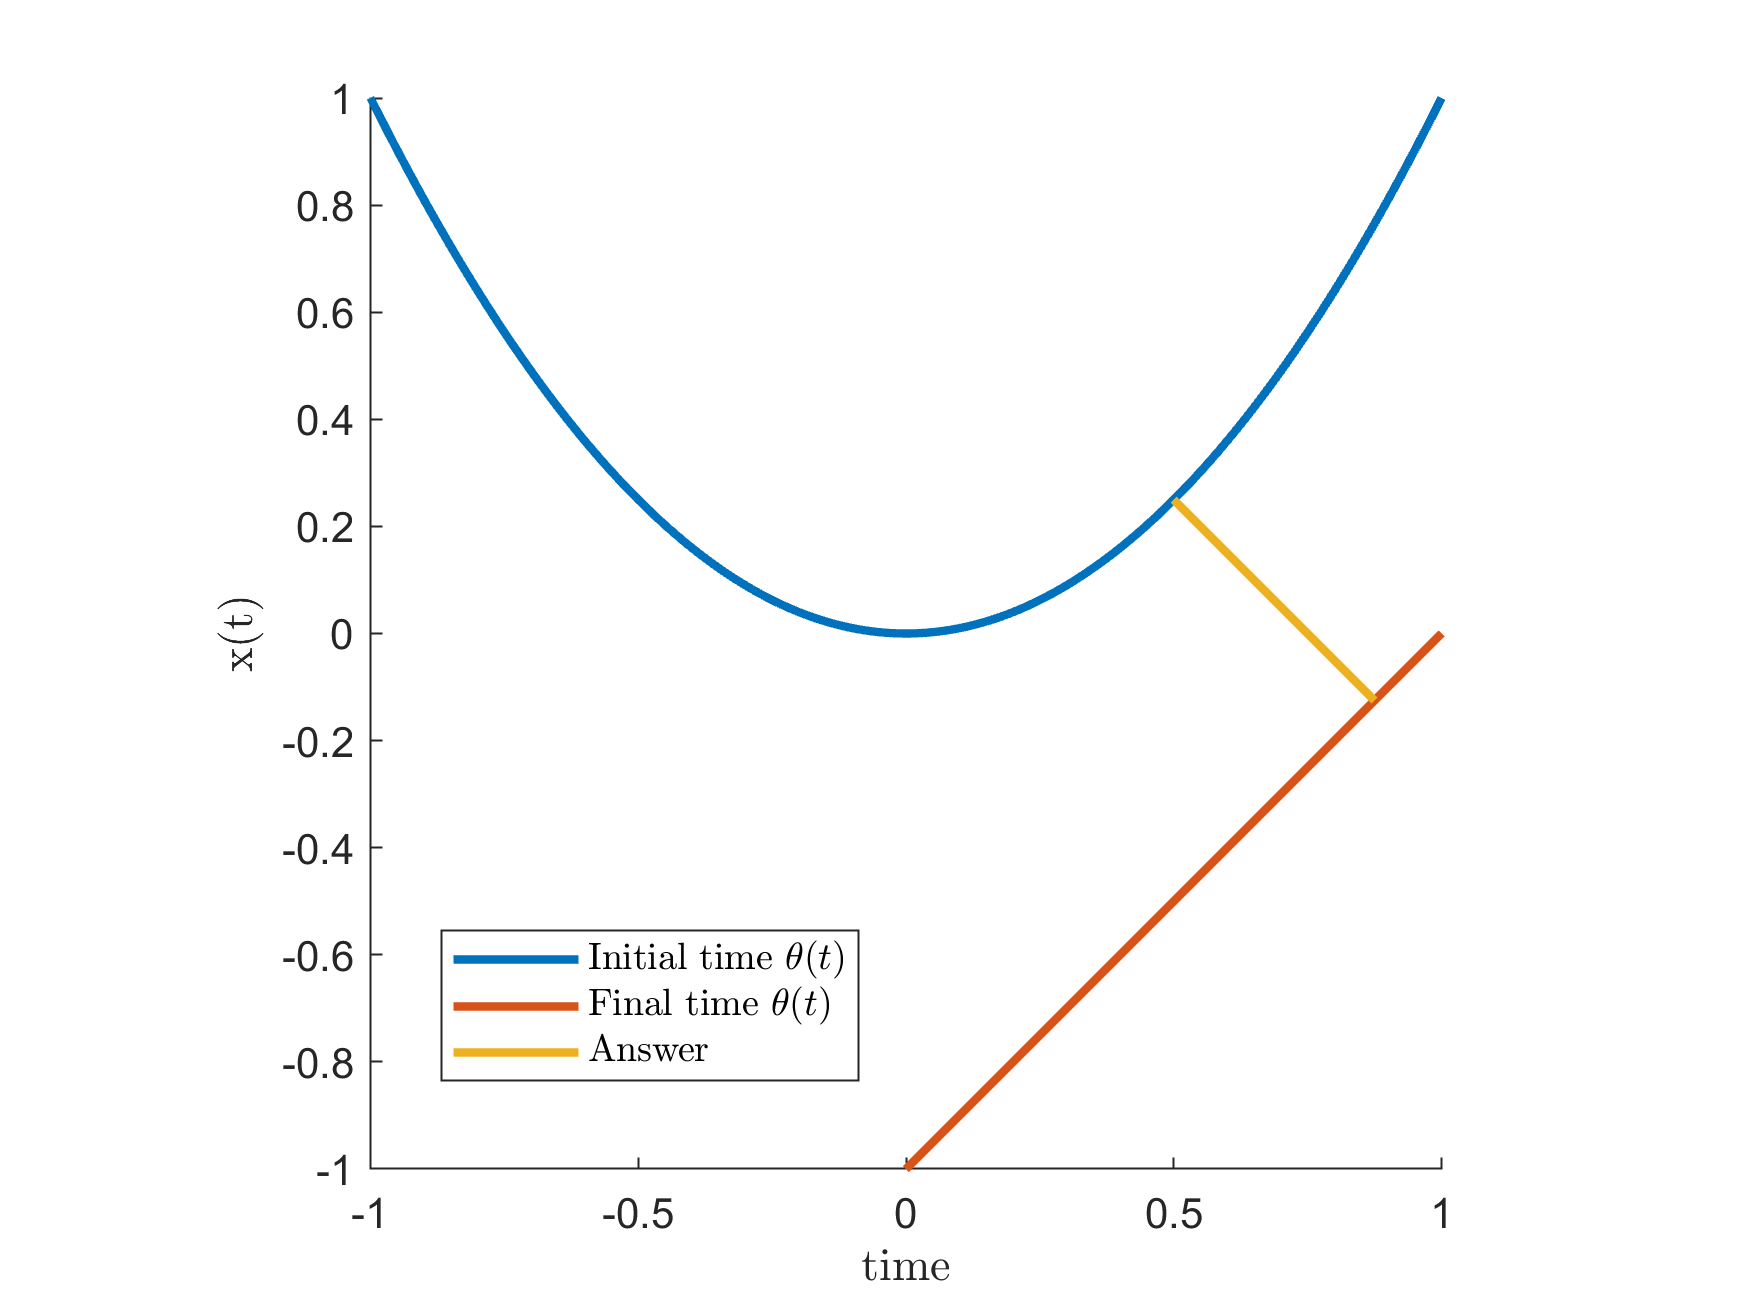
\includegraphics[width=12cm]{Q3/figures/Q3figureFix.png}
\end{figure}
